\chapter{State of Art}
\label{chapter:StateOfArt}

\section{Open Data}
\label{section:OpenData}

Both public and private sectors produce a wide variety of information of interest for citizens and businesses, such as social, economic, geographic, statistical, meteorological, tourism, business and education information. This data has characteristics that make it particularly attractive to the digital content sector, as it is complete, reliable, and of high quality. There are many areas where we can expect this data to be valuable, and where examples of how it has been used already exist. Many different groups of people and organizations can also benefit from the availability of open data, including the public administrations themselves, but at the same time, it is impossible to predict precisely how and where value will be created in the future.

The openness of public sector data allows any person or organization to build on it a new idea that results in new data, knowledge, improve processes, add value to existing ones or even create new services. Consequently, it has considerable economic potential and also favors transparency, participation and citizen collaboration, which are necessary for a more open government.

Open data is data that can be freely used, re-used, and redistributed by anyone - subject only, at most, to the requirement to attribute and share-alike\cite{OpenDataHandbook}.

\subsection{Defining Open}

This paradigm of widely available data has been around since the first years of the internet, with open software in the lead and with the comprehension from most of the entities that form the web, that the share of knowledge always leads to improvements in the common future.

The word Open encompasses a wide range of definitions and nuances, but in this case, when we talk about open knowledge, it is important to correctly define what we are really referring to.

“Open means anyone can freely access, use, modify, and share for any purpose (subject, at most, to requirements that preserve provenance and openness).” \cite{what-is-open}

\subsection{Open Smart Cities}

While massive data collection through sensors attached to physical infrastruc-tures (or Big Data) had always been a characteristic feature of first-generation smart cities, publishing such data as open data or integrating with the open data published by city authorities on different aspects of city management and life is a relatively recent phenomenon. Actually, one of the main concerns related with the opening of data is individual privacy \cite{CONRADIE2014S10}, but this has been overcome in many ways. 

This seemingly shallow change can open the door for a great number of innovations, and lead to projects that could change how we live and interact with the cities themselves. Despite the short history of open data, there is evidence that it can significantly contribute to open government and transparency, citizens engagement, better-informed decisions,better services, innovative applications, and consequently new businesses and jobs.

Publishing Open Data extracted from different sources like traffic, pollution (not only air pollution, but also acoustic or luminous), public transport services use, affluence of popular public zones, etc, can lead to new solutions developed by individuals or companies, and also new material to research for academics, and consequently, have a positive impact in the city and the life of its inhabitants \cite{ojo2015tale}.

\subsection{Linked Data}

The term "Linked Data" refers to a set of best practices for publishing and connecting structured data on the Web. The web was built with the “Linked” concept from the beginning, with the creation of HTML and the “web” as we know it. However, in recent years the Web has evolved from a global information space of linked documents to one where both documents and data are linked \cite{bizer2011linked}.
Linked data is a set of best practices for ensuring that all data attributes can be easily compared when coming from a multitude of separate data sources, which could have a different idea as to what each attribute means. For example, when two data entities have a name attribute how can the computer be certain that it refers to a "Name of a thing" in the same sense. JSON-LD  introduces the concept of the context element, which provides additional information allowing the computer to interpret the rest of the data with more clarity and depth. But this doesn’t imply that this data should be freely accessible. That is where Open Linked Data comes in. 

Open Linked Data is data that the user can link from various sources, institutions, or organizations, and then explore and combine freely and without restrictions. It is also structured in an agreed format, as RFD, or JSON-LD, extended by NGSI-LD.

\clearpage

\section{Fiware}
\label{section:Fiware}

FIWARE \cite{fiware} is an open software platform promoted by the European ICT industry and the European Commission and developed inside the Future Internet Program (FI-PPP), that provides tools for developing smart solutions, and forms an innovation ecosystem for entrepreneurs to create new applications and services on the Internet. 

The FIWARE platform provides Smart Cloud capabilities, enhanced with a set of tools and libraries called Generic Enablers (GEs). These offer standardized and open APIs that facilitate tasks such as integrating Internet of Things devices, analyzing and processing medium and large scale data (Big Data), or incorporating advanced interfaces to interact with users. The generic enables provided by FIWARE can be classified into different categories, the most important being Context management, IoT, Robots and third-party systems, Context data processing, analysis and visualization, and Access management, publishing and monetization of APIs and context data.

\begin{figure}[H]
	\centering
	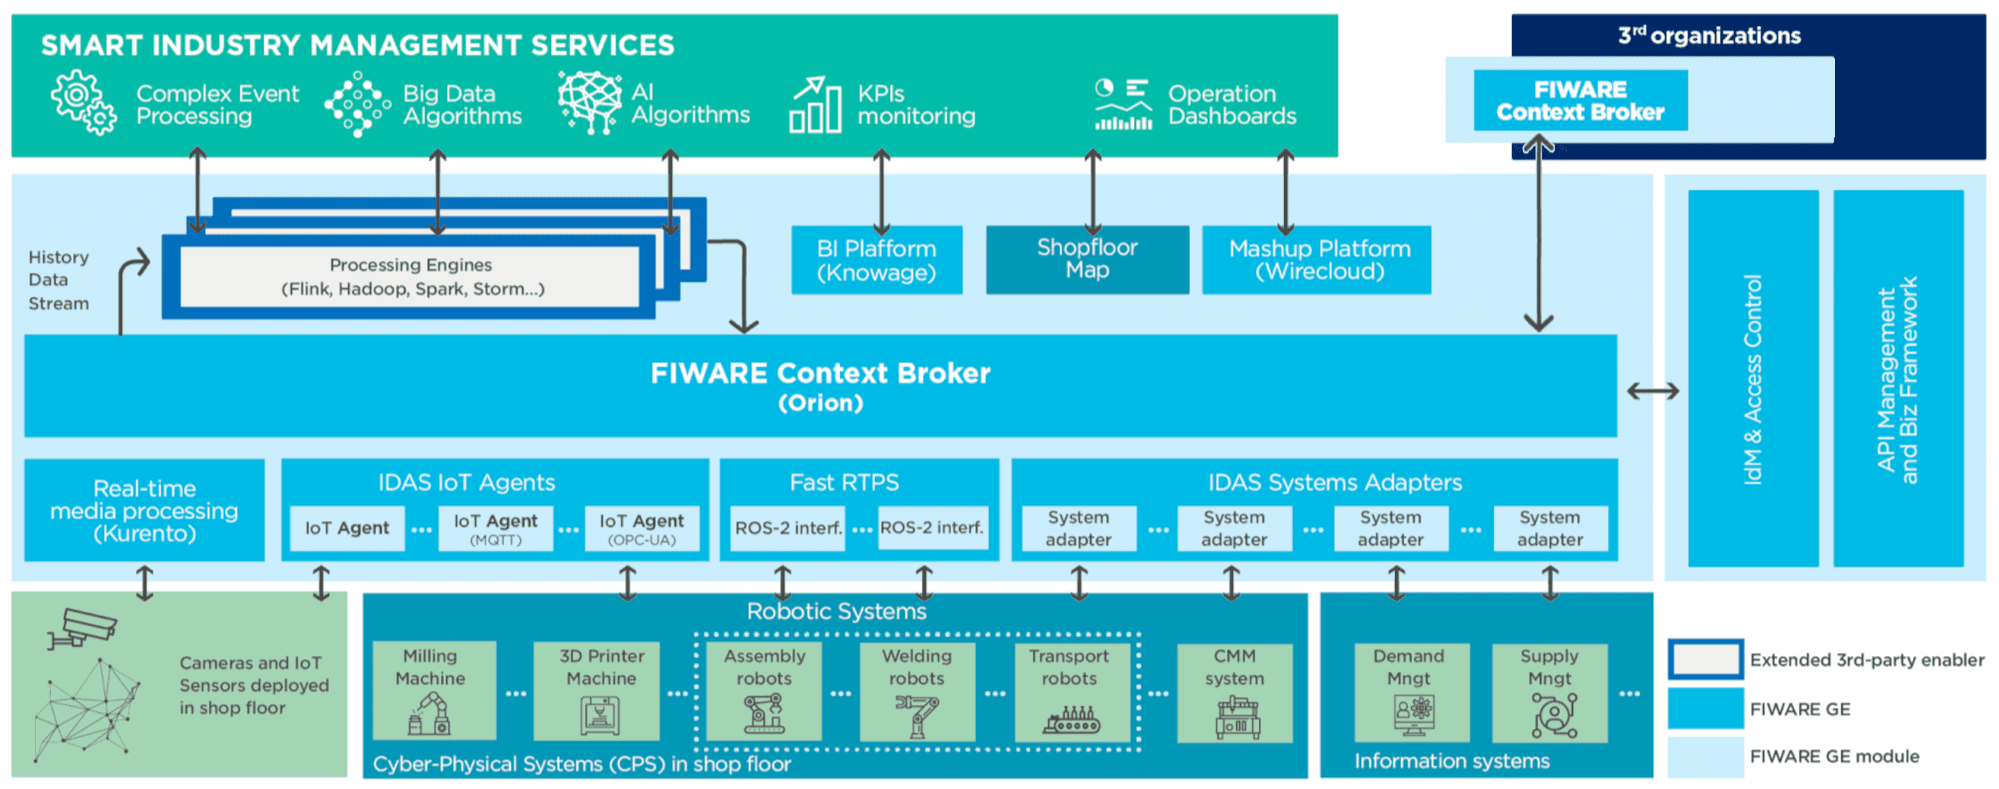
\includegraphics[width=1\linewidth]{imagenes/fiware-architecture.png}
	\caption{Diagram representing the main components of the FIWARE ecosystem. \cite{fiware-docs}}
	\label{fiware-architecture}
\end{figure}

Although FIWARE is a general-purpose platform, it is of special interest in the field of smart cities, due to the appropriateness of the technologies it provides and the importance of the innovation ecosystem in this environment. Since the beginning of the project, FIWARE has worked with a number of cities across Europe to validate and adapt its capabilities to the needs of a smart city, and functional platforms with a big IoT devices deployment has been executed in cities like Helsinki, Amsterdam, Torino, Lisbon, Santander, Seville, Málaga or Valencia between others.

When it comes to the publication and consumption of data, FIWARE  provides the \textbf{NGSI API}, which allows applications to make requests about the context and subscribe to changes in the context, which will be received through notifications. This is useful for example for real-time publication and consumption of sensor data or municipal services.

NGSI v2 is the new standard proposed by FIWARE to manage the context information, and in terms of the data model, properties can be seen as the combination of an attribute and its value. Relationships allow establishing associations between instances using linked data.

\begin{figure}[H]
	\centering
	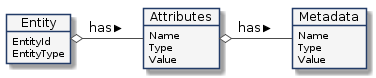
\includegraphics[width=0.8\linewidth]{imagenes/ngsi-v2.png}
	\caption{NGSIv2 entities schema. \cite{fiware-docs}}
	\label{ngsi-v2}
\end{figure}

The core element of NGSI v2 is the data entity, typically a real object with a changing state (such as a Room, a Building, and so on). Entities have attributes (such as name and temperature) and these, in turn, hold metadata such as a timestamp where the measure was taken. Every entity must have a type that defines the sort of thing the entity describes. Relationships can also be defined using NGSI v2, but only so far as giving the attribute an appropriate attribute name.

The core component of a FIWARE platform is the \textbf{Orion Context Broker}. Context information can come from many different sources: existing systems, users with a mobile application, sensor networks, etc. The Context Broker allows modeling and accessing context information regardless of the source of that information, and using its NGSI API, we can interact with the entities and subscriptions created inside it.

Another remarkable GE that we will use in this project is \textbf{Draco}, that is used to persist context data into third-party databases, creating a historical view of the context. It uses Apache NIFI in the background, and because of this, is really powerful for creating data pipelines from our Context Broker to our Database.

Besides the Context broker and Draco, most of the Generic Enablers provided by FIWARE acts as interfaces to hide the underlying complexity of the existing IoT protocols and adapt them to easily integrate with the platform.

\clearpage

\section{Kubernetes}
\label{section:Kubernetes}

Kubernetes \cite{kubernetes} was born as an internal container orchestration solution developed by Google. It is later presented as an open-source project in 2014, joined by large organizations such as Microsoft, Red Hat, IBM, Docker, Openshift, or Huawei.

Kubernetes has established itself as the leading container orchestrator. It allows orchestrating containers from a wide variety of different runtimes, not just Docker. In addition, some of the features that Kubernetes provides are a service discovery system, rollouts and rollbacks, resource optimization on nodes, secret configuration, horizontal scaling of our applications, and many more tools that allow huge and really optimized deployments on top of it. As a container orchestrator, it is designed to work in a declarative way, where instead of giving it the steps to reach a state, we indicate the state in which we want the service to deploy. An example of this is its management with the pods, minimal units of Kubernetes that will be discussed later, when one dies (event), it automatically raises another, provided it is indicated accurately enough.

Broadly speaking, the Kubernetes architecture is divided in two key elements, the master nodes, and the worker nodes. The master node is the entity that coordinates and manages the worker nodes in its cluster, where the containers run. , in the following diagram, the Kubernetes architecture is represented in more detail.


\begin{figure}[H]
	\centering
	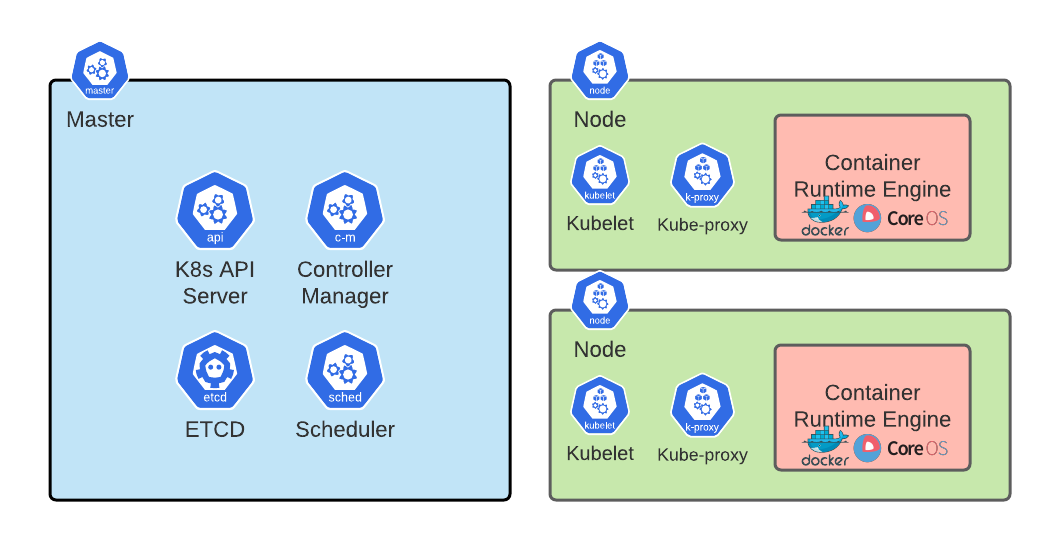
\includegraphics[width=1\linewidth]{imagenes/kubernetes-components.png}
	\caption{Kubernetes general architecture diagram.}
	\label{kubernetes-components}
\end{figure}

The main components of Kubernetes control plane \cite{cka-course}, represented in the previous diagram, have the following function:
\begin{itemize}
\item \textbf{ETCD}:  ETCD is a key-value store used by Kubernetes in order to store it's configuration and on-running information.

\item \textbf{Kube Controller Manager}: It manages the different controllers of Kubernetes. Controllers are like the brain of our cluster and are continuously monitoring the state of various components within the system, and working to maintain the desired functioning state of each one.

\item \textbf{Kube-Scheduler}: Primary management controller in Kubernetes. It manages the communication and management along the rest of the Kubernetes components, it is at the center of all the different tasks related to the cluster.

\item \textbf{Kube-API Server}: Decides which Pod goes on each Node. It doesn't place the pod on the Node though, this is the work of the kubelet of each node. The criteria used for this is based on certain condition: CPU Requirements, Memory resources, Rank function, labels, etc.

\item \textbf{Kubelet}: Kubelet is like the captain of each worker ship. It registers each node scheduled from the scheduler, creates the pods, and informs the master about the status and performance of each node. 

\item \textbf{Kube-proxy}: Pod networking solution to connect the Pods of the different nodes, making use of the Services. The Kube-proxy is a service that runs in each Worker node, and maintains an IP table of services, to route the connections of the different Pods, independently of the node.

\item \textbf{Pod}: A pod is a single instance of an application, and the smallest object that you can create in Kubernetes. A Pod usually contains a single container, and adds Kubernetes-related context to the actual container.
\end{itemize}

Besides the control components and the Pods, there are a lot of resources and objects that Kubernetes will put at our disposal to configure and deploy our applications on Kubernetes. Among them, we will use PersistentVolumes, Services, Deployments, StatefulSets, ReplicaSets or CronJobs.

Other tools designed to work with Kubernetes that we will use in this project are:

\textbf{Minikube}

Minikube \cite{minikube} is a tool created for deploying Kubernetes in your local machine. It uses Docker or any virtual machine environment to set up a single node cluster, this means that the control plane is in the same node that the application containers, but in a different namespace.

\textbf{Kubectl}

Kubectl is the command-line tool provided by Kubernetes to interact with our cluster. It allows us to inspect the cluster, create resources both in imperative and declarative mode.


\section{Machine Learning and Apache Spark}
\label{section:ML}

Machine learning is a branch of artificial intelligence that allows machines to learn without being specifically programmed to do so. By feeding the algorithm with data, it is able to recognize patterns and once trained, generate predictions on new data.

The original definition of Machine Learning, described it as “The field of machine learning is concerned with the question of how to construct computer programs that automatically improve with experience.” \cite{mitchell1997machine},but this definition is too generic, and nowadays with the great advances in both computation and applied statistics, the field has grown huge, we need to be more specific. For the scope of this project, we are not using models from several fields of the Machine Learning world, as Unsupervised Machine Learning or Deep Learning, so we will stick to this definition of the basic Supervised Machine Learning or Predictive modeling: “Find a model or procedure that makes best use of historical data comprised of inputs and outputs in order to skillfully predict outputs given new and unseen inputs in the future.” \cite{brownlee_2019}.

\subsection{Machine Learning Algorithms}

If we want to classify the most popular machine learning algorithms, we can group them by learning style or by similarity. By learning style, that means by how the interact with the input data, we can distinguish the Supervised, Semi-Supervised and Unsupervised categories.

\begin{itemize}
	\item \textbf{Supervised Learning}: Input data is called training data and has a known label or result such as spam/not-spam or a stock price at a time.
	\item \textbf{Unsupervised Learning}: Input data is not labeled and does not have a known result.
	\item \textbf{Semi-Supervised Learning}: Input data is a mixture of labeled and unlabelled examples.
\end{itemize}

\begin{figure}[H]
	\centering
	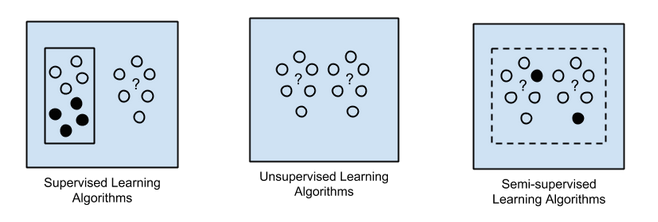
\includegraphics[width=1\linewidth]{imagenes/ml-algos.png}
	\caption{Main classification of ML algorithm by learning style.}
	\label{ml-algos}
\end{figure}

Algorithms related to Machine Learning are often also grouped by similarity in terms of their function (how they work). This generally seems like a more useful way of classifying them, because they also take into account the type of machine learning problem we are trying to solve (Regression and Classification).

Some of the more popular categories, with some examples, are: 

\begin{itemize}
	\item \textbf{Regression Algorithms:}:  They model the relationship between variables that is iteratively refined using a measure of the error in the predictions made by the model. (Linear Regressors, Logistic Regressors, Ordinary Least Squares Regression, etc).
	\item \textbf{Instance-based Algorithms}: Decision problem with instances or examples of training data that are deemed important or required to the model. (Kn-Neighbors, Locally Weighted Learning, Support Vector Machines)
	\item \textbf{Semi-Supervised Learning}: Input data is a mixture of labeled and unlabelled examples.
	\item \textbf{Decision Tree Algorithms}: These methods construct a model of decisions made based on actual values of attributes in the data. (Classification and Regression Tree, Decision Trees).
	\item \textbf{Artificial Neural Network and Deep Learning Algorithms}: These are models that are inspired by the structure and/or function of biological neural networks, and exploit abundant cheap computation. (Multi-Layer Perceptron, Stochastic Gradient Descent, Convolutional Neural Networks, Recurrent Neural Networks).
	\item \textbf{Ensemble Algorithms}: These are models composed of multiple weaker models that are 
	independently trained and whose predictions are combined in some way to make the overall prediction. (AdaBoost, Gradient Boosted Regression Trees, Random Forest).
\end{itemize}

Through the development of this project, we will some of these algorithms from different categories to compare which fits our problem and our data better.
 
\subsection{Apache Spark}

Apache Spark \cite{spark} is a programming framework for processing big data in a distributed manner, designed to be fast. Spark, unlike similar systems as Hadoop, doesn't store any data but loads them in memory for achieving a faster performance. This also makes Spark a really resource-consuming tool, and running it on top of Kubernetes is a good solution for making it more efficient.

Because it was created for being really good at performing tasks in parallel, it is usually deployed in a cluster mode, where a master node will run the main program and distribute the tasks on the worker nodes or executors. It includes APIs for Java, Scala, Python, and R and high-level tools like Spark SQL that allow working with all kinds of integrated functions and with good processing speeds.

The primary abstraction object provided by Spark is a resilient distributed dataset (RDD), which is a collection of partitioned elements between cluster nodes that can be operated on in parallel. RDDs are created by starting from a file or from an existing Scala collection in the driver program, and transforming it. Users can also ask Spark to persist an RDD in memory, allowing it to be efficiently reused through parallel operations, and convert them in DataFrames compatible with other use cases, like pandas DataFrames.

\begin{figure}[H]
	\centering
	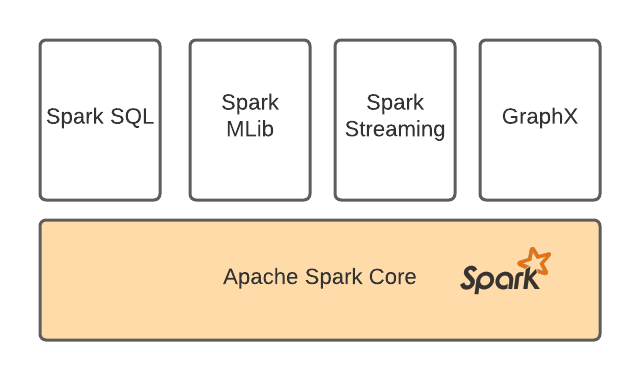
\includegraphics[width=1\linewidth]{imagenes/spark-core.png}
	\caption{Spark main modules and tools.}
	\label{spark-core}
\end{figure}

Some of the more popular tools in the Spark Environment, including the Spark Core itself, are:


\begin{itemize}
	\item \textbf{Spark Core}: This is the core of the Spark framework that supports the other modules.
	\item \textbf{Spark SQL}: Module for processing structured and semi-structured data.
	\item \textbf{MLlib}: Machine Learning library with various types of algorithms such as regression, classification, etc.
	\item \textbf{GraphX}: Graph processing (DAG).
	\item \textbf{Spark Streaming}: Real-time data processing.
\end{itemize}

In the development chapter (\ref{chapter:DesignAndImplementation}), we will explain in more detail how the Spark Cluster works and how to deploy applications on top of it.